\section{Maze and multi-agent exploration}
\label{section_models_maze}
For simulation purposes, this work modeled a maze under an interrelated cells perspective, where each cell is a square with its edges composed by a wall or not. If there is a wall, an agent cannot traverse the maze across the related edge. On the other hand, if there is not a wall, an agent has a free way to traverse the maze through the related edge. It is worth to mention that, if an edge has a wall, the edge of the adjacent corresponding cell also has necessarily a wall.

The maze has a goal that is a single marked cell, and an agent inside the maze aims to find the marked cell, traversing the maze cell by cell. This agent is an autonomous entity that follows a specific algorithm according the current explored path and its programmed initial rules. So that it doesn't go through the same path more than one time, it stores the visited cells. Thus, every time the agent find a branched cell (a cell with at least one edge without a wall), it ignores the already visited branches by itself, and, if there is not a candidate to be a possible branch, the agent go back to the previous visited cell. Furthermore, specifically to this research, differently from some approaches presented in \citen{Beisel2014}, \citen{Burgard2005}, and \citen{KivelevitchCohen2010}, there is no intercommunication between agents in a multi-agent situation to solve the maze.

\citen{Muhammad2021} developed an open-source maze generator. It is a python module that creates randomly mazes and enables the user to simulate its own maze-solving algorithm. In this context, this work presents a multi-agent maze-solving algorithm that has been simulated over \citen{Muhammad2021} open-source code, with modifications. The Figure \ref{maze_model} presents, for example, 2 agents traversing a $6 \times 6$ maze toward the goal.

\citen{Muhammad2021} software creates by default a ``perfect maze'', which means that there is one and only one path to the goal from any cell. However, it is possible to set the code to generate a imperfect maze.

\begin{figure}[ht!]
\centering
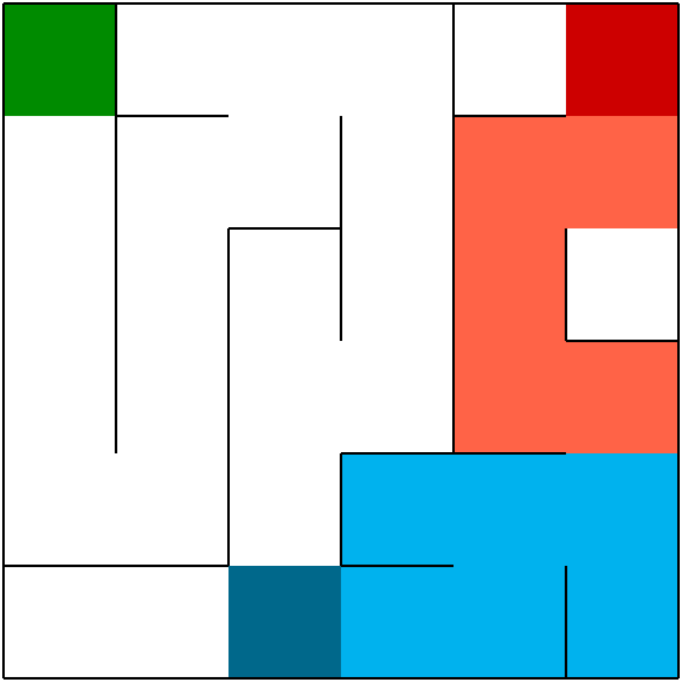
\includegraphics[width=0.5\textwidth]{Cap2/maze_model.png}
\caption{Blue and red agents traversing a $6\times 6$ maze. The goal is represented by the green entity. This maze is a perfect maze \cite{Muhammad2021}.}
\label{maze_model}
\end{figure}

\section{Maze from a graph topology perspective}
\label{section_models_maze_graph}
As pointed out in Section \ref{section_models_maze}, given that an agent ignores visited cells, there is one important point related to this work: if there is only one path to the goal from the agent's initial cell, it is valid to consider a maze as a tree, i.e., a perfect maze \cite{Muhammad2021}. However, if there is more than one path to the goal from the agent's initial cell, the maze cannot be considered as a tree, but it might be considered as a graph.

COLOCAR UMA ÁRVORE REPRESENTANDO UM LABIRINTO 3X3	

\section{Mixed radix representation of the agent path}
\label{section_models_mixed_radix}

\section{Multi-agent exploration without communication}
\label{section_models_mixed_radix}